\documentclass[10pt]{beamer}
\usepackage[utf8]{inputenc}

\usetheme[progressbar=frametitle]{metropolis}
\usepackage{appendixnumberbeamer}

\usepackage{booktabs}
\usepackage[scale=2]{ccicons}
\usepackage{graphicx}
\usepackage{pgfplots}
\usepgfplotslibrary{dateplot}

\usepackage[table]{xcolor}
\usepackage{colortbl}

\usepackage{xspace}
\newcommand{\themename}{\textbf{\textsc{metropolis}}\xspace}


\definecolor{CanvasBG}{HTML}{FAFAFA}

% From the official style guide
\definecolor{UnccGreen}{HTML}{005035}
\definecolor{UnccLightGreen}{HTML}{C3D7A4}
\definecolor{UnccGold}{HTML}{c1d7fe}
\definecolor{UnccOrange}{HTML}{F3901D}
\definecolor{UnccLightYellow}{HTML}{899064}
\definecolor{UnccBlue}{HTML}{007377}
\definecolor{UnccPink}{HTML}{DE3A6E}
\definecolor{White}{HTML}{FFFFFF}
\definecolor{LightGray}{HTML}{F1E6B2}
\definecolor{Purple}{HTML}{6c5098}
\definecolor{Bordeau}{HTML}{570514}
\definecolor{ULB_blue}{HTML}{003087}

\setbeamercolor{frametitle}{bg=ULB_blue}
\setbeamercolor{progress bar}{bg=UnccGold, fg=ULB_blue}
\setbeamercolor{alerted text}{fg=UnccOrange}

\setbeamercolor{block title}{bg=UnccGreen, fg=White}
\setbeamercolor{block title example}{bg=UnccBlue, fg=White}
\setbeamercolor{block title alerted}{bg=UnccPink, fg=White}
\setbeamercolor{block body}{bg=LightGray}

\metroset{titleformat=smallcaps}

% progressbar=foot}

\makeatletter
\setlength{\metropolis@progressinheadfoot@linewidth}{2pt}
\setlength{\metropolis@titleseparator@linewidth}{2pt}
\setlength{\metropolis@progressonsectionpage@linewidth}{2pt}




\title{Mémoire master sciences physiques}
\subtitle{Étude de spectres infrarouges de géantes rouges évoluées}
% \date{\today}
\date{}
\author{\small Margaux Vandererven}
\institute{\small Supervisé par Sophie Van Eck}
 \titlegraphic{\hfill\includegraphics[height=1.5cm]{/Users/margauxvandererven/Documents/unif2023-2024/spectre_IR/rapport/figures/science.png}}

\begin{document}

\maketitle

% \metroset{titleformat frame=allcaps}

\begin{frame}[fragile]{Étoiles de type S \& étoiles à baryum}

    \begin{columns}
            \begin{column}{0.5\textwidth}
                    T$_{\text{eff}}$ étoiles S $\sim$ T$_{\text{eff}}$ étoiles K et M \\

                    Bande ZrO \& enrichissement en éléments s \\
    					\begin{itemize}
    						\item de type S intrinsèques (Tc rich)
    						\item de type S extrinsèques (Tc poor)
    						\item à baryum
    						\item[] 
    					\end{itemize} 
            \end{column}
            \begin{column}{0.5\textwidth}
                \centering
                \includegraphics[width=\textwidth]{/Users/margauxvandererven/Documents/unif2023-2024/spectre_IR/rapport/figures/agb_structure.jpeg}
    			% \caption{\textit{Structure interne d'une étoile AGB}}
            \end{column}
    \end{columns}
\end{frame}

% \metroset{titleformat frame=allcaps}
\begin{frame}[fragile]{Processus s}
    % \begin{columns}
    %     \begin{column}{0.3\textwidth}
    %         +50\% éléments plus lourds que le fer \\
    %     \end{column}
    %     \begin{column}{0.7\textwidth}
    %         \centering
    %         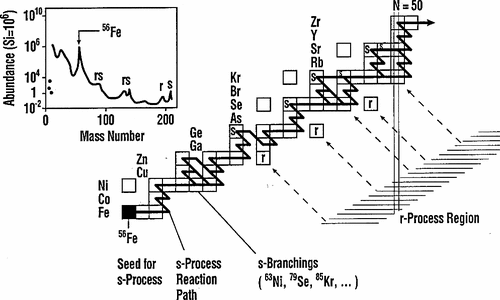
\includegraphics[width=8cm]{images/medium.png}
    %     \end{column}
    % \end{columns}

    \begin{center}
        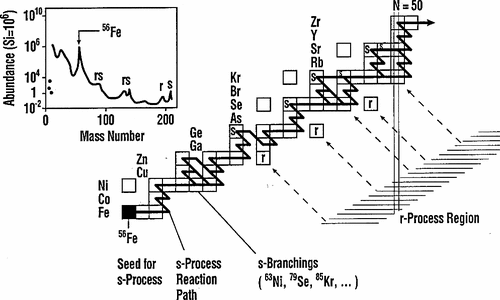
\includegraphics[width=10cm]{images/medium.png} \\
        + de 50\% éléments plus lourds que le fer \\
    \end{center}
\end{frame}

% \metroset{titleformat frame=allcaps}
\begin{frame}[fragile]{Spectre observé}
% \begin{columns}
%     \begin{column}{0.3\textwidth}
             Spectres infrarouges : \\
             IGRINS (Immersion GRating INfrared Spectrometer) \\ 
             Haute résolution : R=$\frac{\lambda}{\Delta \lambda}$ $\sim$ 45000 \\
    					\begin{itemize}
    						\item Bande H (1.45 - 1.80 $\mu m$)
    						\item Bande K (2.05 - 2.50 $\mu m$)
    						\item[]
    					\end{itemize}
        $\rightarrow$ BD-2217$^{\circ}$42 (4000K) \\
        \vfill
        Normalisation \& correction redshift
%     \end{column}
% \end{columns}
\end{frame}

\begin{frame}[fragile]{Etoiles}
    % \begin{column}{0.7\textwidth}
        \begin{table}[h!]
        %     % \caption{Étoiles et paramètres d'atmosphère stellaire}
                \begin{center}
                \resizebox{\textwidth}{!}{
                \begin{tabular}{cccccc}
                    \hline
                    \hline
                     Étoile & Type spectral & $T_{\rm eff}$ (K) & log $g$ (cm $s^{-2}$) & $\xi_{\rm micro}$ (km s$^{-1}$) & [Fe/H] (dex) \\
                    \hline
                    HD 60197 & K3.5III:Ba3.5 & $3800\pm50^{(3)}$ & $2.00\pm0.50^{(3)}$ & $2.00^{(3)}$ & $-0.60\pm0.20^{(3)}$\\
                    HD 63733 & 	S3.5/3 & $3700^{(1)}$ & $1.00^{(1)}$ & - & $-0.10\pm0.13^{(1)}$ \\
                    CR Cir & S6,2  & - & - & - & - \\
                    HD 123949 & K1pBa & $4378\pm80^{(3)}$ & $1.78\pm0.53^{(3)}$ & $1.37^{(3)}$ & $-0.31\pm0.13^{(3)}$ \\
                    \cellcolor{red!15}BD-22$^{\circ}$1742 & \cellcolor{red!15}S3:*3& \cellcolor{red!15}$4000^{(1)}$ & \cellcolor{red!15}$1.00^{(1)}$ & \cellcolor{red!15}- & \cellcolor{red!15}$-0.30\pm0.09^{(1)}$ \\
                    CD-29$^{\circ}$5912 & S4,4 & $3600^{(4)}$ & $1.00^{(4)}$ & - & $-0.40\pm0.22^{(4)}$ \\
                    BD-18$^{\circ}$2608 & S & $3500^{(2)}$ & $1.00^{(2)}$ & - & $-0.31\pm0.16^{(2)}$ \\
                    HD 116869 & G8III:Ba1 & $4892\pm30^{(3)}$ & $2.59\pm0.07^{(3)}$ & $1.38\pm0.04^{(3)}$ & $-0.44\pm0.09^{(3)}$ \\
                    HD 120620 & K0III (Ba$^{(3)}$) & $4831\pm13^{(3)}$ & $3.03\pm0.30^{(3)}$ & $1.11\pm0.05^{(3)}$ & $-0.30\pm0.10^{(3)}$ \\
                    HD 121447 & K4III$^{(3)}$ (Ba$^{(3)}$) & $4000\pm50^{(3)}$ & $1.00\pm0.50^{(3)}$ & $2.00^{(3)}$ & $-0.90\pm0.13^{(3)}$\\
                    HD 100503 & G/KpBa & $4000\pm50^{(3)}$ & $2.00\pm0.50^{(3)}$ & $2.00^{(3)}$ & $-0.72\pm0.13^{(3)}$ \\
                    HD 119185 &  G8IIIpBa & - & - & - & - \\
                    HD 88562  & K1III (Ba$^{(3)}$)& $4000\pm50^{(3)}$ & $2.00\pm0.50^{(3)}$ & $2.00^{(3)}$ & $-0.53\pm0.12^{(3)}$\\
                    V812 Oph  & S5+/2.5 & $3500^{(2)}$ & $1.00^{(2)}$ & - & $-0.37\pm0.13^{(2)}$\\
                    19 Aql  & F0III-IV & - & - & - & -  \\
                    V915 Aql  & S5+/2 & $3400^{(1)}$ & $0.00^{(1)}$ & - & $-0.50\pm0.15^{(1)}$ \\
                    HD 165774 & S4,6 & - & - & - & - \\
                    \hline
                \end{tabular}}
                \end{center}
        %     % \textbf{Notes}. Le type spectral est majoritairement repris de SIMBAD ; la première lettre faisant référence au système Harvard (O,B,A, F, G, K, M), le chiffre arabe suivant à la nomenclature "early"/"late", le chiffre romain à la classe de luminosité, "Ba" pour étoile à baryum / "S" pour étoile de type S et la lettre minuscule faisant référence aux particularités du spectre (par exemple, "p" pour "particularité non spécifiée").
            
            % \textbf{Références}. $^{(1)}$\cite{shetye_s_2018}, $^{(2)}$\cite{shetye_s_2021} , $^{(3)}$\cite{karinkuzhi_when_2018}, $^{(4)}$\cite{shetye_observational_2019}.
        %     %     \label{param_stellaire}
            \end{table}
    % \end{column}
\end{frame}

\begin{frame}[fragile]{Spectre synthétique}
    \begin{columns}
        \begin{column}{0.5\textwidth}
            \begin{center}
                TurboSpectrum v20 
            \end{center}
        \end{column}
        \begin{column}{0.5\textwidth}
            \begin{center}
                MARCS 
            \end{center}
        \end{column}
\end{columns}
\end{frame}

% \metroset{titleformat frame=allcaps}
\begin{frame}[fragile]{Contributions moléculaires}
  
\begin{table}
    %    \caption{}
        \begin{tabular}{c|ccc}
            \toprule
        \midrule
            &Molécules & Bande H (\%) & Bande K (\%)\\
            \midrule
            \textbf{Cat. I}&$^{12}$C$^{14}$N & 82.47 & 76.33  \\
            \small($>$ 10\%)&$^{13}$C$^{14}$N & 78.52 & 67.18  \\
            &$^{12}$C$^{16}$O & 71.92 & 71.01   \\
            &HF & 1.81 & 47.39   \\
            &$^{12}$C$^{12}$C & 81.40 & 77.39  \\
            &$^{12}$C$^{13}$C & 73.81  & 65.34   \\
            \textbf{Cat. II}&$^{13}$C$^{13}$C & 7.84  & 3.51  \\
            \small(1-10\%)&$^{16}$OH & 2.20  & 0.56    \\
            &$^{56}$FeH & 2.96  & 0.08   \\
            &$^{12}$CH & 5.97  & 8.55   \\
            \bottomrule
        \end{tabular}
\end{table}
\textbf{Cat. III} ($<$ 1\%) : $^{13}$C$^{17}$O, $^{13}$CH, $^{14}$NH, $^{48}$TiO, C$_{2}$H$_2$, HCl, H$_{2}$O, $^{20}$CaH, $^{28}$SiH, $^{28}$SiO, VO, YO, $^{48}$TiO, $^{24}$MgH, AlH, $^{52}$CrH, H$^{12}$CN, H$^{13}$CN, $^{90-94}$ZrO et $^{96}$ZrO
\end{frame}


% \metroset{titleformat frame=allcaps}
\begin{frame}[fragile]{Abondances C, N, O}

\textbf{Abondances} : 
	\begin{table}
    		\begin{tabular}{c|cccc}
      		\toprule
			\midrule
       		&$[Fe/H]$ & $[C/Fe]$ & $[N/Fe]$&$ [O/Fe]$\\
      		\midrule
			\textit{Ce travail} & - & 0.41 &0.32 & 0.75  \\
      		\textit{Shetye et al. (2018)} &-0.30$\pm$0.09& 0.35 &-0.1 &-  \\
            \bottomrule
    		\end{tabular}
	  \end{table}

\end{frame}

\begin{frame}[fragile]{Paramètres stellaires}
    dd
\end{frame}

% \begin{frame}[fragile]{Références}
%     % \bibliographystyle{plain}
%     % \bibliography{bibtex.bib}
% \end{frame}

\end{document}